\chapter{Background}
\label{chap:background}
This chapter introduces the necessary background information for this study. First, a thorough description of the Transformer model is provided in \cref{sec:transformer}. \cref{sec:metrics} explain the different metrics used in this thesis, followed by a brief introduction to blockchain technology in \cref{sec:blockchain}. Then, the concept of \acrfullpl{sc} and the most popular \acrshort{sc} vulnerabilities are described in \cref{sec:smart-contract}.

\section{Transformer}
\label{sec:transformer}
A transformer is a deep learning model. It is designed to process sequential data and adopts the mechanism of self-attention. The Transformer model architecture was introduced in \citeyear{vaswani2017attention} by \textcite{vaswani2017attention}. Unlike more traditional attention-based models such as \acrfullpl{rnn}, transformers do not include any recurrence or convolutions. This allows the model to process the entire input all at once, solely relying on attention. It solves the vanishing gradient problem of recurrent models, where long-range dependencies within the input are not accurately captured. It also allows the model to be significantly more parallelized, making training on huge datasets feasible. Because of this, pre-trained systems such as \acrfull{bert} \cite{devlin2018bert} and \acrshort{gpt} \cite{radford2018improving} were developed. These models are pre-trained on a large corpus of text, such as Wikipedia Corpus and Common Crawl, and effectively predict the next word in a sentence. Further, the models can be fine-tuned on a new dataset to improve their performance on more specialized tasks.

\subsection{Architecture}
\label{sec:transformer-architecture}
The standard Transformer architecture, as described by \textcite{vaswani2017attention} in \citeyear{vaswani2017attention}, is shown in \cref{fig:transformer-architecture}. The following subsections describe the architecture of the standard Transformer model.

\begin{figure}[htp]
    \centering
    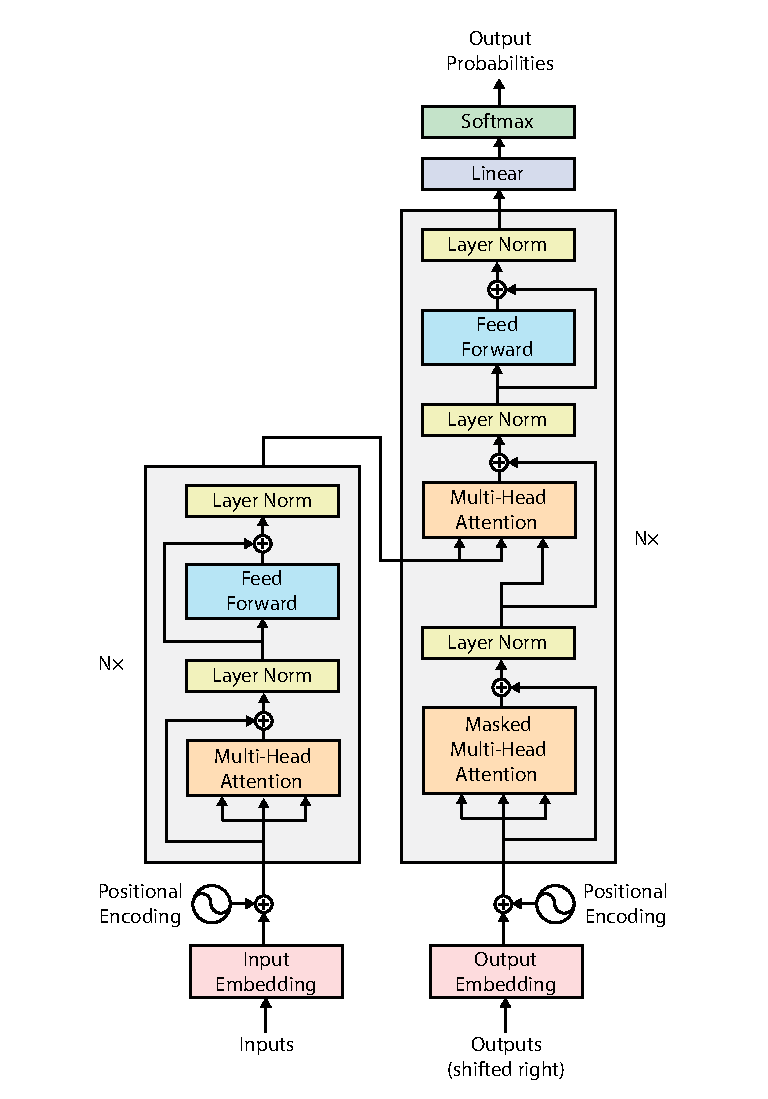
\includegraphics[width=0.8\textwidth]{figures/transformer_architecture.pdf}
    \caption{Architecture of a standard Transformer \textcite{vaswani2017attention}}
    \label{fig:transformer-architecture}
\end{figure}


\subsubsection{Tokenization}
\label{sec:tokenization}
For a Transformer to process the text input, the text is first tokenized. Tokenization is the process of breaking a sequence of text into a sequence of tokens. For example, the sentence \textit{I am a sentence.} is tokenized into the words "\textit{I}", "\textit{am}", "\textit{a}", "\textit{sentence}", and "\textit{.}". The tokenization process is usually done by a tokenizer. Specifically, the transformer uses a byte pair encoding tokenizer.

\subsubsection{Embedding and Positional Encoding}
\label{sec:embedding-and-positional-encoding}
After the input text is tokenized, the next step for the model is to understand the meaning and position of the token (word) in the sequence. This is achieved by an Embedding layer and a Positional encoding layer. The results of these two layers are combined.

Two embedding layers are used. The Input Embedding layer is fed the input sequence. The Output Embedding layer accepts the target sequence after shifting the target to the right by one position and inserting a start token at the first position. The embedding layers produce a numerical representation of the input sequence, mapping each token to an embedding vector.

\begin{figure}[htp]
    \centering
    %% Creator: Matplotlib, PGF backend
%%
%% To include the figure in your LaTeX document, write
%%   \input{<filename>.pgf}
%%
%% Make sure the required packages are loaded in your preamble
%%   \usepackage{pgf}
%%
%% and, on pdftex
%%   \usepackage[utf8]{inputenc}\DeclareUnicodeCharacter{2212}{-}
%%
%% or, on luatex and xetex
%%   \usepackage{unicode-math}
%%
%% Figures using additional raster images can only be included by \input if
%% they are in the same directory as the main LaTeX file. For loading figures
%% from other directories you can use the `import` package
%%   \usepackage{import}
%%
%% and then include the figures with
%%   \import{<path to file>}{<filename>.pgf}
%%
%% Matplotlib used the following preamble
%%
\begingroup%
\makeatletter%
\begin{pgfpicture}%
\pgfpathrectangle{\pgfpointorigin}{\pgfqpoint{4.840359in}{2.401102in}}%
\pgfusepath{use as bounding box, clip}%
\begin{pgfscope}%
\pgfsetbuttcap%
\pgfsetmiterjoin%
\definecolor{currentfill}{rgb}{1.000000,1.000000,1.000000}%
\pgfsetfillcolor{currentfill}%
\pgfsetlinewidth{0.000000pt}%
\definecolor{currentstroke}{rgb}{1.000000,1.000000,1.000000}%
\pgfsetstrokecolor{currentstroke}%
\pgfsetdash{}{0pt}%
\pgfpathmoveto{\pgfqpoint{0.000000in}{-0.000000in}}%
\pgfpathlineto{\pgfqpoint{4.840359in}{-0.000000in}}%
\pgfpathlineto{\pgfqpoint{4.840359in}{2.401102in}}%
\pgfpathlineto{\pgfqpoint{0.000000in}{2.401102in}}%
\pgfpathclose%
\pgfusepath{fill}%
\end{pgfscope}%
\begin{pgfscope}%
\pgfsetbuttcap%
\pgfsetmiterjoin%
\definecolor{currentfill}{rgb}{1.000000,1.000000,1.000000}%
\pgfsetfillcolor{currentfill}%
\pgfsetlinewidth{0.000000pt}%
\definecolor{currentstroke}{rgb}{0.000000,0.000000,0.000000}%
\pgfsetstrokecolor{currentstroke}%
\pgfsetstrokeopacity{0.000000}%
\pgfsetdash{}{0pt}%
\pgfpathmoveto{\pgfqpoint{0.584568in}{0.499691in}}%
\pgfpathlineto{\pgfqpoint{4.053193in}{0.499691in}}%
\pgfpathlineto{\pgfqpoint{4.053193in}{2.252877in}}%
\pgfpathlineto{\pgfqpoint{0.584568in}{2.252877in}}%
\pgfpathclose%
\pgfusepath{fill}%
\end{pgfscope}%
\begin{pgfscope}%
\pgfsys@transformshift{0.584167in}{0.500269in}%
\pgftext[left,bottom]{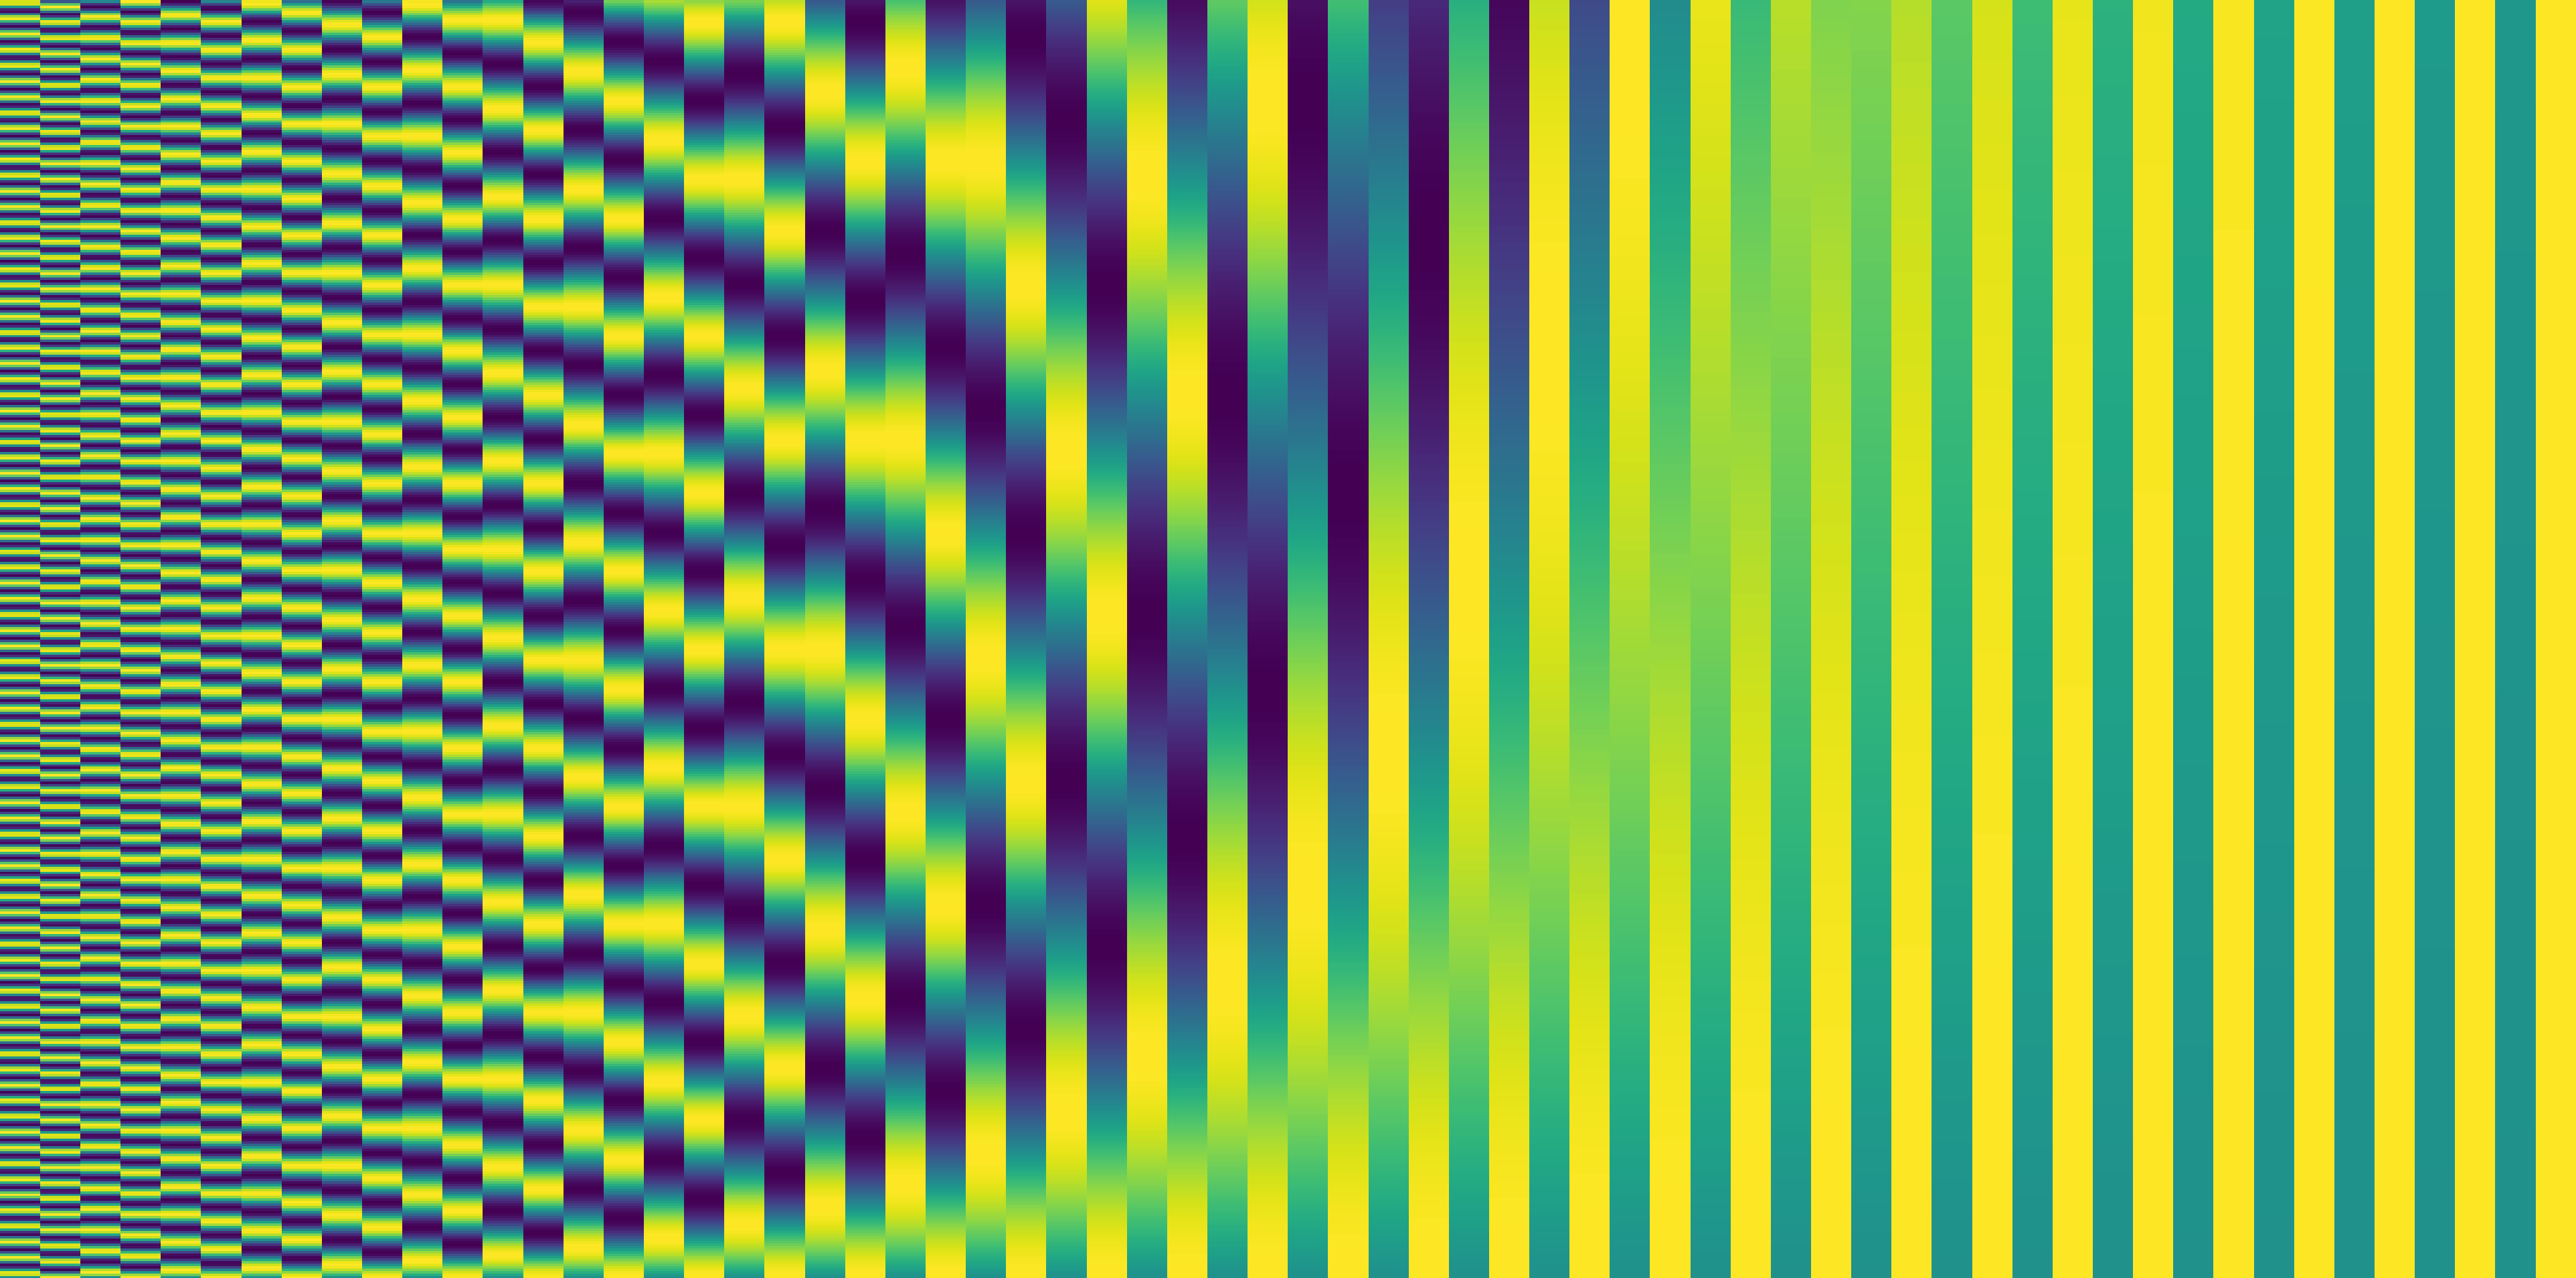
\includegraphics[interpolate=true,width=3.469167in,height=1.752500in]{figures/positional_embedding-img0.png}}%
\end{pgfscope}%
\begin{pgfscope}%
\pgfsetbuttcap%
\pgfsetroundjoin%
\definecolor{currentfill}{rgb}{0.000000,0.000000,0.000000}%
\pgfsetfillcolor{currentfill}%
\pgfsetlinewidth{0.803000pt}%
\definecolor{currentstroke}{rgb}{0.000000,0.000000,0.000000}%
\pgfsetstrokecolor{currentstroke}%
\pgfsetdash{}{0pt}%
\pgfsys@defobject{currentmarker}{\pgfqpoint{0.000000in}{-0.048611in}}{\pgfqpoint{0.000000in}{0.000000in}}{%
\pgfpathmoveto{\pgfqpoint{0.000000in}{0.000000in}}%
\pgfpathlineto{\pgfqpoint{0.000000in}{-0.048611in}}%
\pgfusepath{stroke,fill}%
}%
\begin{pgfscope}%
\pgfsys@transformshift{0.584568in}{0.499691in}%
\pgfsys@useobject{currentmarker}{}%
\end{pgfscope}%
\end{pgfscope}%
\begin{pgfscope}%
\definecolor{textcolor}{rgb}{0.000000,0.000000,0.000000}%
\pgfsetstrokecolor{textcolor}%
\pgfsetfillcolor{textcolor}%
\pgftext[x=0.584568in,y=0.402469in,,top]{\color{textcolor}\rmfamily\fontsize{10.000000}{12.000000}\selectfont \(\displaystyle {0}\)}%
\end{pgfscope}%
\begin{pgfscope}%
\pgfsetbuttcap%
\pgfsetroundjoin%
\definecolor{currentfill}{rgb}{0.000000,0.000000,0.000000}%
\pgfsetfillcolor{currentfill}%
\pgfsetlinewidth{0.803000pt}%
\definecolor{currentstroke}{rgb}{0.000000,0.000000,0.000000}%
\pgfsetstrokecolor{currentstroke}%
\pgfsetdash{}{0pt}%
\pgfsys@defobject{currentmarker}{\pgfqpoint{0.000000in}{-0.048611in}}{\pgfqpoint{0.000000in}{0.000000in}}{%
\pgfpathmoveto{\pgfqpoint{0.000000in}{0.000000in}}%
\pgfpathlineto{\pgfqpoint{0.000000in}{-0.048611in}}%
\pgfusepath{stroke,fill}%
}%
\begin{pgfscope}%
\pgfsys@transformshift{1.126541in}{0.499691in}%
\pgfsys@useobject{currentmarker}{}%
\end{pgfscope}%
\end{pgfscope}%
\begin{pgfscope}%
\definecolor{textcolor}{rgb}{0.000000,0.000000,0.000000}%
\pgfsetstrokecolor{textcolor}%
\pgfsetfillcolor{textcolor}%
\pgftext[x=1.126541in,y=0.402469in,,top]{\color{textcolor}\rmfamily\fontsize{10.000000}{12.000000}\selectfont \(\displaystyle {10}\)}%
\end{pgfscope}%
\begin{pgfscope}%
\pgfsetbuttcap%
\pgfsetroundjoin%
\definecolor{currentfill}{rgb}{0.000000,0.000000,0.000000}%
\pgfsetfillcolor{currentfill}%
\pgfsetlinewidth{0.803000pt}%
\definecolor{currentstroke}{rgb}{0.000000,0.000000,0.000000}%
\pgfsetstrokecolor{currentstroke}%
\pgfsetdash{}{0pt}%
\pgfsys@defobject{currentmarker}{\pgfqpoint{0.000000in}{-0.048611in}}{\pgfqpoint{0.000000in}{0.000000in}}{%
\pgfpathmoveto{\pgfqpoint{0.000000in}{0.000000in}}%
\pgfpathlineto{\pgfqpoint{0.000000in}{-0.048611in}}%
\pgfusepath{stroke,fill}%
}%
\begin{pgfscope}%
\pgfsys@transformshift{1.668514in}{0.499691in}%
\pgfsys@useobject{currentmarker}{}%
\end{pgfscope}%
\end{pgfscope}%
\begin{pgfscope}%
\definecolor{textcolor}{rgb}{0.000000,0.000000,0.000000}%
\pgfsetstrokecolor{textcolor}%
\pgfsetfillcolor{textcolor}%
\pgftext[x=1.668514in,y=0.402469in,,top]{\color{textcolor}\rmfamily\fontsize{10.000000}{12.000000}\selectfont \(\displaystyle {20}\)}%
\end{pgfscope}%
\begin{pgfscope}%
\pgfsetbuttcap%
\pgfsetroundjoin%
\definecolor{currentfill}{rgb}{0.000000,0.000000,0.000000}%
\pgfsetfillcolor{currentfill}%
\pgfsetlinewidth{0.803000pt}%
\definecolor{currentstroke}{rgb}{0.000000,0.000000,0.000000}%
\pgfsetstrokecolor{currentstroke}%
\pgfsetdash{}{0pt}%
\pgfsys@defobject{currentmarker}{\pgfqpoint{0.000000in}{-0.048611in}}{\pgfqpoint{0.000000in}{0.000000in}}{%
\pgfpathmoveto{\pgfqpoint{0.000000in}{0.000000in}}%
\pgfpathlineto{\pgfqpoint{0.000000in}{-0.048611in}}%
\pgfusepath{stroke,fill}%
}%
\begin{pgfscope}%
\pgfsys@transformshift{2.210486in}{0.499691in}%
\pgfsys@useobject{currentmarker}{}%
\end{pgfscope}%
\end{pgfscope}%
\begin{pgfscope}%
\definecolor{textcolor}{rgb}{0.000000,0.000000,0.000000}%
\pgfsetstrokecolor{textcolor}%
\pgfsetfillcolor{textcolor}%
\pgftext[x=2.210486in,y=0.402469in,,top]{\color{textcolor}\rmfamily\fontsize{10.000000}{12.000000}\selectfont \(\displaystyle {30}\)}%
\end{pgfscope}%
\begin{pgfscope}%
\pgfsetbuttcap%
\pgfsetroundjoin%
\definecolor{currentfill}{rgb}{0.000000,0.000000,0.000000}%
\pgfsetfillcolor{currentfill}%
\pgfsetlinewidth{0.803000pt}%
\definecolor{currentstroke}{rgb}{0.000000,0.000000,0.000000}%
\pgfsetstrokecolor{currentstroke}%
\pgfsetdash{}{0pt}%
\pgfsys@defobject{currentmarker}{\pgfqpoint{0.000000in}{-0.048611in}}{\pgfqpoint{0.000000in}{0.000000in}}{%
\pgfpathmoveto{\pgfqpoint{0.000000in}{0.000000in}}%
\pgfpathlineto{\pgfqpoint{0.000000in}{-0.048611in}}%
\pgfusepath{stroke,fill}%
}%
\begin{pgfscope}%
\pgfsys@transformshift{2.752459in}{0.499691in}%
\pgfsys@useobject{currentmarker}{}%
\end{pgfscope}%
\end{pgfscope}%
\begin{pgfscope}%
\definecolor{textcolor}{rgb}{0.000000,0.000000,0.000000}%
\pgfsetstrokecolor{textcolor}%
\pgfsetfillcolor{textcolor}%
\pgftext[x=2.752459in,y=0.402469in,,top]{\color{textcolor}\rmfamily\fontsize{10.000000}{12.000000}\selectfont \(\displaystyle {40}\)}%
\end{pgfscope}%
\begin{pgfscope}%
\pgfsetbuttcap%
\pgfsetroundjoin%
\definecolor{currentfill}{rgb}{0.000000,0.000000,0.000000}%
\pgfsetfillcolor{currentfill}%
\pgfsetlinewidth{0.803000pt}%
\definecolor{currentstroke}{rgb}{0.000000,0.000000,0.000000}%
\pgfsetstrokecolor{currentstroke}%
\pgfsetdash{}{0pt}%
\pgfsys@defobject{currentmarker}{\pgfqpoint{0.000000in}{-0.048611in}}{\pgfqpoint{0.000000in}{0.000000in}}{%
\pgfpathmoveto{\pgfqpoint{0.000000in}{0.000000in}}%
\pgfpathlineto{\pgfqpoint{0.000000in}{-0.048611in}}%
\pgfusepath{stroke,fill}%
}%
\begin{pgfscope}%
\pgfsys@transformshift{3.294432in}{0.499691in}%
\pgfsys@useobject{currentmarker}{}%
\end{pgfscope}%
\end{pgfscope}%
\begin{pgfscope}%
\definecolor{textcolor}{rgb}{0.000000,0.000000,0.000000}%
\pgfsetstrokecolor{textcolor}%
\pgfsetfillcolor{textcolor}%
\pgftext[x=3.294432in,y=0.402469in,,top]{\color{textcolor}\rmfamily\fontsize{10.000000}{12.000000}\selectfont \(\displaystyle {50}\)}%
\end{pgfscope}%
\begin{pgfscope}%
\pgfsetbuttcap%
\pgfsetroundjoin%
\definecolor{currentfill}{rgb}{0.000000,0.000000,0.000000}%
\pgfsetfillcolor{currentfill}%
\pgfsetlinewidth{0.803000pt}%
\definecolor{currentstroke}{rgb}{0.000000,0.000000,0.000000}%
\pgfsetstrokecolor{currentstroke}%
\pgfsetdash{}{0pt}%
\pgfsys@defobject{currentmarker}{\pgfqpoint{0.000000in}{-0.048611in}}{\pgfqpoint{0.000000in}{0.000000in}}{%
\pgfpathmoveto{\pgfqpoint{0.000000in}{0.000000in}}%
\pgfpathlineto{\pgfqpoint{0.000000in}{-0.048611in}}%
\pgfusepath{stroke,fill}%
}%
\begin{pgfscope}%
\pgfsys@transformshift{3.836404in}{0.499691in}%
\pgfsys@useobject{currentmarker}{}%
\end{pgfscope}%
\end{pgfscope}%
\begin{pgfscope}%
\definecolor{textcolor}{rgb}{0.000000,0.000000,0.000000}%
\pgfsetstrokecolor{textcolor}%
\pgfsetfillcolor{textcolor}%
\pgftext[x=3.836404in,y=0.402469in,,top]{\color{textcolor}\rmfamily\fontsize{10.000000}{12.000000}\selectfont \(\displaystyle {60}\)}%
\end{pgfscope}%
\begin{pgfscope}%
\definecolor{textcolor}{rgb}{0.000000,0.000000,0.000000}%
\pgfsetstrokecolor{textcolor}%
\pgfsetfillcolor{textcolor}%
\pgftext[x=2.318881in,y=0.223457in,,top]{\color{textcolor}\rmfamily\fontsize{10.000000}{12.000000}\selectfont Depth}%
\end{pgfscope}%
\begin{pgfscope}%
\pgfsetbuttcap%
\pgfsetroundjoin%
\definecolor{currentfill}{rgb}{0.000000,0.000000,0.000000}%
\pgfsetfillcolor{currentfill}%
\pgfsetlinewidth{0.803000pt}%
\definecolor{currentstroke}{rgb}{0.000000,0.000000,0.000000}%
\pgfsetstrokecolor{currentstroke}%
\pgfsetdash{}{0pt}%
\pgfsys@defobject{currentmarker}{\pgfqpoint{-0.048611in}{0.000000in}}{\pgfqpoint{0.000000in}{0.000000in}}{%
\pgfpathmoveto{\pgfqpoint{0.000000in}{0.000000in}}%
\pgfpathlineto{\pgfqpoint{-0.048611in}{0.000000in}}%
\pgfusepath{stroke,fill}%
}%
\begin{pgfscope}%
\pgfsys@transformshift{0.584568in}{0.499691in}%
\pgfsys@useobject{currentmarker}{}%
\end{pgfscope}%
\end{pgfscope}%
\begin{pgfscope}%
\definecolor{textcolor}{rgb}{0.000000,0.000000,0.000000}%
\pgfsetstrokecolor{textcolor}%
\pgfsetfillcolor{textcolor}%
\pgftext[x=0.417902in, y=0.451466in, left, base]{\color{textcolor}\rmfamily\fontsize{10.000000}{12.000000}\selectfont \(\displaystyle {0}\)}%
\end{pgfscope}%
\begin{pgfscope}%
\pgfsetbuttcap%
\pgfsetroundjoin%
\definecolor{currentfill}{rgb}{0.000000,0.000000,0.000000}%
\pgfsetfillcolor{currentfill}%
\pgfsetlinewidth{0.803000pt}%
\definecolor{currentstroke}{rgb}{0.000000,0.000000,0.000000}%
\pgfsetstrokecolor{currentstroke}%
\pgfsetdash{}{0pt}%
\pgfsys@defobject{currentmarker}{\pgfqpoint{-0.048611in}{0.000000in}}{\pgfqpoint{0.000000in}{0.000000in}}{%
\pgfpathmoveto{\pgfqpoint{0.000000in}{0.000000in}}%
\pgfpathlineto{\pgfqpoint{-0.048611in}{0.000000in}}%
\pgfusepath{stroke,fill}%
}%
\begin{pgfscope}%
\pgfsys@transformshift{0.584568in}{0.842110in}%
\pgfsys@useobject{currentmarker}{}%
\end{pgfscope}%
\end{pgfscope}%
\begin{pgfscope}%
\definecolor{textcolor}{rgb}{0.000000,0.000000,0.000000}%
\pgfsetstrokecolor{textcolor}%
\pgfsetfillcolor{textcolor}%
\pgftext[x=0.279012in, y=0.793885in, left, base]{\color{textcolor}\rmfamily\fontsize{10.000000}{12.000000}\selectfont \(\displaystyle {100}\)}%
\end{pgfscope}%
\begin{pgfscope}%
\pgfsetbuttcap%
\pgfsetroundjoin%
\definecolor{currentfill}{rgb}{0.000000,0.000000,0.000000}%
\pgfsetfillcolor{currentfill}%
\pgfsetlinewidth{0.803000pt}%
\definecolor{currentstroke}{rgb}{0.000000,0.000000,0.000000}%
\pgfsetstrokecolor{currentstroke}%
\pgfsetdash{}{0pt}%
\pgfsys@defobject{currentmarker}{\pgfqpoint{-0.048611in}{0.000000in}}{\pgfqpoint{0.000000in}{0.000000in}}{%
\pgfpathmoveto{\pgfqpoint{0.000000in}{0.000000in}}%
\pgfpathlineto{\pgfqpoint{-0.048611in}{0.000000in}}%
\pgfusepath{stroke,fill}%
}%
\begin{pgfscope}%
\pgfsys@transformshift{0.584568in}{1.184529in}%
\pgfsys@useobject{currentmarker}{}%
\end{pgfscope}%
\end{pgfscope}%
\begin{pgfscope}%
\definecolor{textcolor}{rgb}{0.000000,0.000000,0.000000}%
\pgfsetstrokecolor{textcolor}%
\pgfsetfillcolor{textcolor}%
\pgftext[x=0.279012in, y=1.136304in, left, base]{\color{textcolor}\rmfamily\fontsize{10.000000}{12.000000}\selectfont \(\displaystyle {200}\)}%
\end{pgfscope}%
\begin{pgfscope}%
\pgfsetbuttcap%
\pgfsetroundjoin%
\definecolor{currentfill}{rgb}{0.000000,0.000000,0.000000}%
\pgfsetfillcolor{currentfill}%
\pgfsetlinewidth{0.803000pt}%
\definecolor{currentstroke}{rgb}{0.000000,0.000000,0.000000}%
\pgfsetstrokecolor{currentstroke}%
\pgfsetdash{}{0pt}%
\pgfsys@defobject{currentmarker}{\pgfqpoint{-0.048611in}{0.000000in}}{\pgfqpoint{0.000000in}{0.000000in}}{%
\pgfpathmoveto{\pgfqpoint{0.000000in}{0.000000in}}%
\pgfpathlineto{\pgfqpoint{-0.048611in}{0.000000in}}%
\pgfusepath{stroke,fill}%
}%
\begin{pgfscope}%
\pgfsys@transformshift{0.584568in}{1.526949in}%
\pgfsys@useobject{currentmarker}{}%
\end{pgfscope}%
\end{pgfscope}%
\begin{pgfscope}%
\definecolor{textcolor}{rgb}{0.000000,0.000000,0.000000}%
\pgfsetstrokecolor{textcolor}%
\pgfsetfillcolor{textcolor}%
\pgftext[x=0.279012in, y=1.478723in, left, base]{\color{textcolor}\rmfamily\fontsize{10.000000}{12.000000}\selectfont \(\displaystyle {300}\)}%
\end{pgfscope}%
\begin{pgfscope}%
\pgfsetbuttcap%
\pgfsetroundjoin%
\definecolor{currentfill}{rgb}{0.000000,0.000000,0.000000}%
\pgfsetfillcolor{currentfill}%
\pgfsetlinewidth{0.803000pt}%
\definecolor{currentstroke}{rgb}{0.000000,0.000000,0.000000}%
\pgfsetstrokecolor{currentstroke}%
\pgfsetdash{}{0pt}%
\pgfsys@defobject{currentmarker}{\pgfqpoint{-0.048611in}{0.000000in}}{\pgfqpoint{0.000000in}{0.000000in}}{%
\pgfpathmoveto{\pgfqpoint{0.000000in}{0.000000in}}%
\pgfpathlineto{\pgfqpoint{-0.048611in}{0.000000in}}%
\pgfusepath{stroke,fill}%
}%
\begin{pgfscope}%
\pgfsys@transformshift{0.584568in}{1.869368in}%
\pgfsys@useobject{currentmarker}{}%
\end{pgfscope}%
\end{pgfscope}%
\begin{pgfscope}%
\definecolor{textcolor}{rgb}{0.000000,0.000000,0.000000}%
\pgfsetstrokecolor{textcolor}%
\pgfsetfillcolor{textcolor}%
\pgftext[x=0.279012in, y=1.821142in, left, base]{\color{textcolor}\rmfamily\fontsize{10.000000}{12.000000}\selectfont \(\displaystyle {400}\)}%
\end{pgfscope}%
\begin{pgfscope}%
\pgfsetbuttcap%
\pgfsetroundjoin%
\definecolor{currentfill}{rgb}{0.000000,0.000000,0.000000}%
\pgfsetfillcolor{currentfill}%
\pgfsetlinewidth{0.803000pt}%
\definecolor{currentstroke}{rgb}{0.000000,0.000000,0.000000}%
\pgfsetstrokecolor{currentstroke}%
\pgfsetdash{}{0pt}%
\pgfsys@defobject{currentmarker}{\pgfqpoint{-0.048611in}{0.000000in}}{\pgfqpoint{0.000000in}{0.000000in}}{%
\pgfpathmoveto{\pgfqpoint{0.000000in}{0.000000in}}%
\pgfpathlineto{\pgfqpoint{-0.048611in}{0.000000in}}%
\pgfusepath{stroke,fill}%
}%
\begin{pgfscope}%
\pgfsys@transformshift{0.584568in}{2.211787in}%
\pgfsys@useobject{currentmarker}{}%
\end{pgfscope}%
\end{pgfscope}%
\begin{pgfscope}%
\definecolor{textcolor}{rgb}{0.000000,0.000000,0.000000}%
\pgfsetstrokecolor{textcolor}%
\pgfsetfillcolor{textcolor}%
\pgftext[x=0.279012in, y=2.163562in, left, base]{\color{textcolor}\rmfamily\fontsize{10.000000}{12.000000}\selectfont \(\displaystyle {500}\)}%
\end{pgfscope}%
\begin{pgfscope}%
\definecolor{textcolor}{rgb}{0.000000,0.000000,0.000000}%
\pgfsetstrokecolor{textcolor}%
\pgfsetfillcolor{textcolor}%
\pgftext[x=0.223457in,y=1.376284in,,bottom,rotate=90.000000]{\color{textcolor}\rmfamily\fontsize{10.000000}{12.000000}\selectfont Position}%
\end{pgfscope}%
\begin{pgfscope}%
\pgfsetrectcap%
\pgfsetmiterjoin%
\pgfsetlinewidth{0.803000pt}%
\definecolor{currentstroke}{rgb}{0.000000,0.000000,0.000000}%
\pgfsetstrokecolor{currentstroke}%
\pgfsetdash{}{0pt}%
\pgfpathmoveto{\pgfqpoint{0.584568in}{0.499691in}}%
\pgfpathlineto{\pgfqpoint{0.584568in}{2.252877in}}%
\pgfusepath{stroke}%
\end{pgfscope}%
\begin{pgfscope}%
\pgfsetrectcap%
\pgfsetmiterjoin%
\pgfsetlinewidth{0.803000pt}%
\definecolor{currentstroke}{rgb}{0.000000,0.000000,0.000000}%
\pgfsetstrokecolor{currentstroke}%
\pgfsetdash{}{0pt}%
\pgfpathmoveto{\pgfqpoint{4.053193in}{0.499691in}}%
\pgfpathlineto{\pgfqpoint{4.053193in}{2.252877in}}%
\pgfusepath{stroke}%
\end{pgfscope}%
\begin{pgfscope}%
\pgfsetrectcap%
\pgfsetmiterjoin%
\pgfsetlinewidth{0.803000pt}%
\definecolor{currentstroke}{rgb}{0.000000,0.000000,0.000000}%
\pgfsetstrokecolor{currentstroke}%
\pgfsetdash{}{0pt}%
\pgfpathmoveto{\pgfqpoint{0.584568in}{0.499691in}}%
\pgfpathlineto{\pgfqpoint{4.053193in}{0.499691in}}%
\pgfusepath{stroke}%
\end{pgfscope}%
\begin{pgfscope}%
\pgfsetrectcap%
\pgfsetmiterjoin%
\pgfsetlinewidth{0.803000pt}%
\definecolor{currentstroke}{rgb}{0.000000,0.000000,0.000000}%
\pgfsetstrokecolor{currentstroke}%
\pgfsetdash{}{0pt}%
\pgfpathmoveto{\pgfqpoint{0.584568in}{2.252877in}}%
\pgfpathlineto{\pgfqpoint{4.053193in}{2.252877in}}%
\pgfusepath{stroke}%
\end{pgfscope}%
\begin{pgfscope}%
\pgfpathrectangle{\pgfqpoint{4.269982in}{0.499691in}}{\pgfqpoint{0.087659in}{1.753186in}}%
\pgfusepath{clip}%
\pgfsetbuttcap%
\pgfsetmiterjoin%
\definecolor{currentfill}{rgb}{1.000000,1.000000,1.000000}%
\pgfsetfillcolor{currentfill}%
\pgfsetlinewidth{0.010037pt}%
\definecolor{currentstroke}{rgb}{1.000000,1.000000,1.000000}%
\pgfsetstrokecolor{currentstroke}%
\pgfsetdash{}{0pt}%
\pgfpathmoveto{\pgfqpoint{4.269982in}{0.499691in}}%
\pgfpathlineto{\pgfqpoint{4.269982in}{0.506539in}}%
\pgfpathlineto{\pgfqpoint{4.269982in}{2.246029in}}%
\pgfpathlineto{\pgfqpoint{4.269982in}{2.252877in}}%
\pgfpathlineto{\pgfqpoint{4.357642in}{2.252877in}}%
\pgfpathlineto{\pgfqpoint{4.357642in}{2.246029in}}%
\pgfpathlineto{\pgfqpoint{4.357642in}{0.506539in}}%
\pgfpathlineto{\pgfqpoint{4.357642in}{0.499691in}}%
\pgfpathclose%
\pgfusepath{stroke,fill}%
\end{pgfscope}%
\begin{pgfscope}%
\pgfsys@transformshift{4.270000in}{0.500269in}%
\pgftext[left,bottom]{
\includegraphics[interpolate=true,width=0.087500in,height=1.752500in]{figures/positional_embedding-img1.png}}%
\end{pgfscope}%
\begin{pgfscope}%
\pgfsetbuttcap%
\pgfsetroundjoin%
\definecolor{currentfill}{rgb}{0.000000,0.000000,0.000000}%
\pgfsetfillcolor{currentfill}%
\pgfsetlinewidth{0.803000pt}%
\definecolor{currentstroke}{rgb}{0.000000,0.000000,0.000000}%
\pgfsetstrokecolor{currentstroke}%
\pgfsetdash{}{0pt}%
\pgfsys@defobject{currentmarker}{\pgfqpoint{0.000000in}{0.000000in}}{\pgfqpoint{0.048611in}{0.000000in}}{%
\pgfpathmoveto{\pgfqpoint{0.000000in}{0.000000in}}%
\pgfpathlineto{\pgfqpoint{0.048611in}{0.000000in}}%
\pgfusepath{stroke,fill}%
}%
\begin{pgfscope}%
\pgfsys@transformshift{4.357642in}{0.499691in}%
\pgfsys@useobject{currentmarker}{}%
\end{pgfscope}%
\end{pgfscope}%
\begin{pgfscope}%
\definecolor{textcolor}{rgb}{0.000000,0.000000,0.000000}%
\pgfsetstrokecolor{textcolor}%
\pgfsetfillcolor{textcolor}%
\pgftext[x=4.454864in, y=0.451466in, left, base]{\color{textcolor}\rmfamily\fontsize{10.000000}{12.000000}\selectfont \(\displaystyle {-1.0}\)}%
\end{pgfscope}%
\begin{pgfscope}%
\pgfsetbuttcap%
\pgfsetroundjoin%
\definecolor{currentfill}{rgb}{0.000000,0.000000,0.000000}%
\pgfsetfillcolor{currentfill}%
\pgfsetlinewidth{0.803000pt}%
\definecolor{currentstroke}{rgb}{0.000000,0.000000,0.000000}%
\pgfsetstrokecolor{currentstroke}%
\pgfsetdash{}{0pt}%
\pgfsys@defobject{currentmarker}{\pgfqpoint{0.000000in}{0.000000in}}{\pgfqpoint{0.048611in}{0.000000in}}{%
\pgfpathmoveto{\pgfqpoint{0.000000in}{0.000000in}}%
\pgfpathlineto{\pgfqpoint{0.048611in}{0.000000in}}%
\pgfusepath{stroke,fill}%
}%
\begin{pgfscope}%
\pgfsys@transformshift{4.357642in}{0.937988in}%
\pgfsys@useobject{currentmarker}{}%
\end{pgfscope}%
\end{pgfscope}%
\begin{pgfscope}%
\definecolor{textcolor}{rgb}{0.000000,0.000000,0.000000}%
\pgfsetstrokecolor{textcolor}%
\pgfsetfillcolor{textcolor}%
\pgftext[x=4.454864in, y=0.889762in, left, base]{\color{textcolor}\rmfamily\fontsize{10.000000}{12.000000}\selectfont \(\displaystyle {-0.5}\)}%
\end{pgfscope}%
\begin{pgfscope}%
\pgfsetbuttcap%
\pgfsetroundjoin%
\definecolor{currentfill}{rgb}{0.000000,0.000000,0.000000}%
\pgfsetfillcolor{currentfill}%
\pgfsetlinewidth{0.803000pt}%
\definecolor{currentstroke}{rgb}{0.000000,0.000000,0.000000}%
\pgfsetstrokecolor{currentstroke}%
\pgfsetdash{}{0pt}%
\pgfsys@defobject{currentmarker}{\pgfqpoint{0.000000in}{0.000000in}}{\pgfqpoint{0.048611in}{0.000000in}}{%
\pgfpathmoveto{\pgfqpoint{0.000000in}{0.000000in}}%
\pgfpathlineto{\pgfqpoint{0.048611in}{0.000000in}}%
\pgfusepath{stroke,fill}%
}%
\begin{pgfscope}%
\pgfsys@transformshift{4.357642in}{1.376284in}%
\pgfsys@useobject{currentmarker}{}%
\end{pgfscope}%
\end{pgfscope}%
\begin{pgfscope}%
\definecolor{textcolor}{rgb}{0.000000,0.000000,0.000000}%
\pgfsetstrokecolor{textcolor}%
\pgfsetfillcolor{textcolor}%
\pgftext[x=4.454864in, y=1.328059in, left, base]{\color{textcolor}\rmfamily\fontsize{10.000000}{12.000000}\selectfont \(\displaystyle {0.0}\)}%
\end{pgfscope}%
\begin{pgfscope}%
\pgfsetbuttcap%
\pgfsetroundjoin%
\definecolor{currentfill}{rgb}{0.000000,0.000000,0.000000}%
\pgfsetfillcolor{currentfill}%
\pgfsetlinewidth{0.803000pt}%
\definecolor{currentstroke}{rgb}{0.000000,0.000000,0.000000}%
\pgfsetstrokecolor{currentstroke}%
\pgfsetdash{}{0pt}%
\pgfsys@defobject{currentmarker}{\pgfqpoint{0.000000in}{0.000000in}}{\pgfqpoint{0.048611in}{0.000000in}}{%
\pgfpathmoveto{\pgfqpoint{0.000000in}{0.000000in}}%
\pgfpathlineto{\pgfqpoint{0.048611in}{0.000000in}}%
\pgfusepath{stroke,fill}%
}%
\begin{pgfscope}%
\pgfsys@transformshift{4.357642in}{1.814581in}%
\pgfsys@useobject{currentmarker}{}%
\end{pgfscope}%
\end{pgfscope}%
\begin{pgfscope}%
\definecolor{textcolor}{rgb}{0.000000,0.000000,0.000000}%
\pgfsetstrokecolor{textcolor}%
\pgfsetfillcolor{textcolor}%
\pgftext[x=4.454864in, y=1.766355in, left, base]{\color{textcolor}\rmfamily\fontsize{10.000000}{12.000000}\selectfont \(\displaystyle {0.5}\)}%
\end{pgfscope}%
\begin{pgfscope}%
\pgfsetbuttcap%
\pgfsetroundjoin%
\definecolor{currentfill}{rgb}{0.000000,0.000000,0.000000}%
\pgfsetfillcolor{currentfill}%
\pgfsetlinewidth{0.803000pt}%
\definecolor{currentstroke}{rgb}{0.000000,0.000000,0.000000}%
\pgfsetstrokecolor{currentstroke}%
\pgfsetdash{}{0pt}%
\pgfsys@defobject{currentmarker}{\pgfqpoint{0.000000in}{0.000000in}}{\pgfqpoint{0.048611in}{0.000000in}}{%
\pgfpathmoveto{\pgfqpoint{0.000000in}{0.000000in}}%
\pgfpathlineto{\pgfqpoint{0.048611in}{0.000000in}}%
\pgfusepath{stroke,fill}%
}%
\begin{pgfscope}%
\pgfsys@transformshift{4.357642in}{2.252877in}%
\pgfsys@useobject{currentmarker}{}%
\end{pgfscope}%
\end{pgfscope}%
\begin{pgfscope}%
\definecolor{textcolor}{rgb}{0.000000,0.000000,0.000000}%
\pgfsetstrokecolor{textcolor}%
\pgfsetfillcolor{textcolor}%
\pgftext[x=4.454864in, y=2.204652in, left, base]{\color{textcolor}\rmfamily\fontsize{10.000000}{12.000000}\selectfont \(\displaystyle {1.0}\)}%
\end{pgfscope}%
\begin{pgfscope}%
\pgfsetbuttcap%
\pgfsetmiterjoin%
\pgfsetlinewidth{0.803000pt}%
\definecolor{currentstroke}{rgb}{0.000000,0.000000,0.000000}%
\pgfsetstrokecolor{currentstroke}%
\pgfsetdash{}{0pt}%
\pgfpathmoveto{\pgfqpoint{4.269982in}{0.499691in}}%
\pgfpathlineto{\pgfqpoint{4.269982in}{0.506539in}}%
\pgfpathlineto{\pgfqpoint{4.269982in}{2.246029in}}%
\pgfpathlineto{\pgfqpoint{4.269982in}{2.252877in}}%
\pgfpathlineto{\pgfqpoint{4.357642in}{2.252877in}}%
\pgfpathlineto{\pgfqpoint{4.357642in}{2.246029in}}%
\pgfpathlineto{\pgfqpoint{4.357642in}{0.506539in}}%
\pgfpathlineto{\pgfqpoint{4.357642in}{0.499691in}}%
\pgfpathclose%
\pgfusepath{stroke}%
\end{pgfscope}%
\end{pgfpicture}%
\makeatother%
\endgroup%

    \caption{The 64-dimensional positional encoding for a sentence with the maximum length of 512. Each row represents an positional encoding vector.}
    \label{fig:positional-embedding}
\end{figure}

The positional encoding is generated by a sinusoidal positional encoding layer. This layer is fed the sequence length and produces a sinusoidal positional encoding vector. This is illustrated in \cref{fig:positional-embedding}, where each row corresponds to one sinusoidal positional encoding vector. The positional encoding vector is then added to the embedding vector.

\subsubsection{Encoder and decoder stacks}
\label{sec:encoder-decoder-stacks}
A Transformer is comprised of two main parts: the encoder and the decoder. The encoder is responsible for encoding the input sequence into a sequence of vectors. It tries to capture information about which parts of the inputs are relevant to each other. The decoder is responsible for decoding the output sequence from the encoder. Along with other inputs, the decoder is optimized for generating outputs. In \cref{fig:transformer-architecture}, the left and right halves represent the Transformer encoder and decoder, respectively. 

The encoder and decoder are both composed of a stack of self-attention layers. This layer allows the model to pay more or less attention to certain words in the input sentence as it is handling a specific word. Each decoder layer has an additional attention mechanism that draws information from the outputs of previous decoders, before the decoder layer draws information from the encodings. Both the encoder and decoder layers contain a feed-forward layer for further processing of the outputs, as well as layer normalization and residual connections.

The transformer architecture allows for auto-regressive text generation. This is achieved by re-feeding the decoder the encoder outputs. The decoder then generates the next word in a loop until the end of the sentence is reached. For this to work, the  Transformer must not be able to use the current or future output to predict an output. The use of a look-ahead mask solves this. The final output from the transformer is generated by feeding the decoder output through a linear layer and a softmax layer. This produces probabilities for each token in the vocabulary and can be used to predict the next token (word).

The encoder and decoder can also be used independently or in combination. The original transformer model described by \textcite{vaswani2017attention} used an encoder-decoder structure. These models are used for generative tasks that also require input, for example, language translation or text summarization. Encoder-only models are used for tasks that are centered around understanding the input, such as sentence classification and named entity recognition. Decoder-only models excel at generative tasks such as text generation.

\begin{figure}[htp]
    \centering
    \begin{subfigure}[b]{0.5\textwidth}
        \centering
        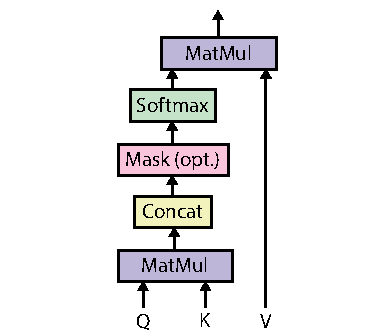
\includegraphics[width=0.8\textwidth,keepaspectratio]{figures/scaled_dot-product_attention.pdf}
        \caption{Scaled Dot-Product Attention.}
        \label{fig:scaled-dotproduct-attention}
    \end{subfigure}%
    \hfill
    \begin{subfigure}[b]{0.5\textwidth}
        \centering
        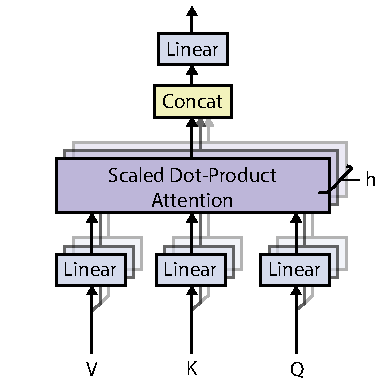
\includegraphics[width=0.8\textwidth,keepaspectratio]{figures/multi-head_attention.pdf}
        \caption{Multi-Head Attention consists of several attention layers running in parallel.}
        \label{fig:multihead-attention}
    \end{subfigure}%
    \caption{Multi-Head Attention module in Transformer architecture \textcite{vaswani2017attention}}
    \label{fig:transformer-architecture-details}
\end{figure}

\subsubsection{Scaled dot-product attention} 
\label{sec:scaled-dot-product-attention}
The self-attention layer used in each Transformer block is named "Scaled Dot-Product Attention". An overview of the attention layer is shown in \cref{fig:scaled-dotproduct-attention}. The layer learns three weight matrices, query weights \(W_Q\), key weights \(W_K\), and value weights \(W_V\). Each input word embedding is multiplied with each weight matrix, producing a query vector, key vector, and value vector. Self-attention scores are then generated by calculating the dot products of the query vector with the key vector of the respective word (query) that is calculated.

In order to stabilize the gradients during training, the attention weights are divided by the square root of the dimension of the key vectors, \(\sqrt{d_{k}}\). A softmax function is then applied, normalizing the scores to be positive and adding up to 1. Each value vector is then multiplied by the softmax score. The resulting weighted value vectors are then summed up and serve as output from the attention layer.

In practice, the attention calculation for all tokens can be expressed as one large matrix calculation, as shown in \cref{fig:scaled-dotproduct-attention}. This significantly speeds up the training process. The queries, keys, and values are packed into the separate matrices \(Q\), \(K\), and \(V\), respectively. The output matrix can be described as:
\begin{equation}
    \text{Attention$(Q,K,V)$} = \text{softmax}(\frac{QK^T}{\sqrt{d_{k}}})V
\end{equation}
where the superscript \(T\) represent the transpose operation.

\subsubsection{Multi-head attention}
\label{sec:multi-head-attention}
By splitting the query, key, and value parameters in N-ways (logically), each with its separate weight matrix, the performance of the Transformer is increased. This is called multi-head attention, illustrated in \cref{fig:multihead-attention}. It gives the Transformer greater power to encode multiple relationships and nuances for each word. The final attention outputs for the feed-forward network are calculated by concatenating the matrixes for each attention head.

\subsection{Training}
\label{sec:transformer-training}
A Transformer model typically undergoes something called self-supervised learning. This is an intermediary between both unsupervised- and supervised learning. This normally conforms to unsupervised pre-training the model on a large set of data. Then, the model is fine-tuned on a (usually) smaller dataset of labeled data.

In contrast to the unsupervised training, where the target sequence comprises the predicted transformer output, the supervised training is done by feeding the complete input- and target language sequence directly into the Transformer. The input sequence is fed to the encoder, while the target sequence is fed to the decoder.

\subsection{Inference}
\label{sec:transformer-inference}
For making inference, the Transformer is only fed the input sequence. The encoder is run on the input sequence, and the encoder output is fed to the decoder. Since no encoder output is available at the first timestep, the decoder is fed a special "<start>" token. The decoder output is then fed back into the decoder again. This process is repeated until the decoder output encounters a special "<stop>" token.

\section{Relevant Metrics}
\label{sec:metrics}

\subsection{Machine learning performance metric}
\label{sec:performance-metric}

\subsubsection{Accuracy}
\label{sec:accuracy}
Accuracy is the proportion of correct predictions among the total number of cases processed \cite{accuracy}. Accuracy is formally defined as the proportion of correct predictions among the total number of cases processed, as seen in \cref{eq:accuracy}.

\begin{equation}
    \label{eq:accuracy}
    \text{Accuracy} = \frac{TP + TN}{TP + TN + FP + FN}
\end{equation}
where \(TP\) is the number of true positives, \(TN\) is the number of true negatives, \(FP\) is the number of false positives, and \(FN\) is the number of false negatives.

It is a very common metric used for evaluating the performance of a machine learning model. However, it has to be used with caution, as an overfitted model would report high accuracy.

\subsubsection{Perplexity}
\label{sec:perplexity}
Perplexity is one of the most common metrics for evaluating language models \cite{perplexity}. It is a measure of how variable a prediction model is, and can be defined as the normalized inverse probability of the test set \cite{perplexity2}. For a test set with words \(W  = w_1, w_2, …, w_N\), the perplexity of the model on the test set is:

\begin{equation}
    \label{eq:perplexity}
    PP(W) = \sqrt[N]{\frac{1}{p(w_1,w_2,...,w_N)}}
\end{equation}

Perplexity can be interpreted as the weighted branching factor. If we have a perplexity of 10, it means that whenever the model tries to guess the next word, it is as confused as if it had to pick between 10 words. Models with lower perplexity have probability values that are more varied. Meaning, the lower perplexity, the better model \cite{perplexity2}.

\subsection{Machine translation performance metrics}
\label{sec:machine-translation-metrics}

\subsubsection{\textsc{Bleu}}
\label{sec:blue-score}
\acrfullr{bleu} by \textcite{papineni2002bleu} is a metric for automatically evaluating machine-translated text. \acrshort{bleu} scores are between 0 and 1. A value of 0 means there is no overlap with the reference translation, while a value of 1 means that the translation perfectly overlaps. A score of 0.6 or 0.7 is considered the best a human can achieve \cite{googlebleu,papineni2002bleu}. The color gradient in \cref{fig:bleu} from \cite{lavie2011evaluating} can be used as a general scale interpretation of the BLEU score.

\begin{figure}
    \centering
    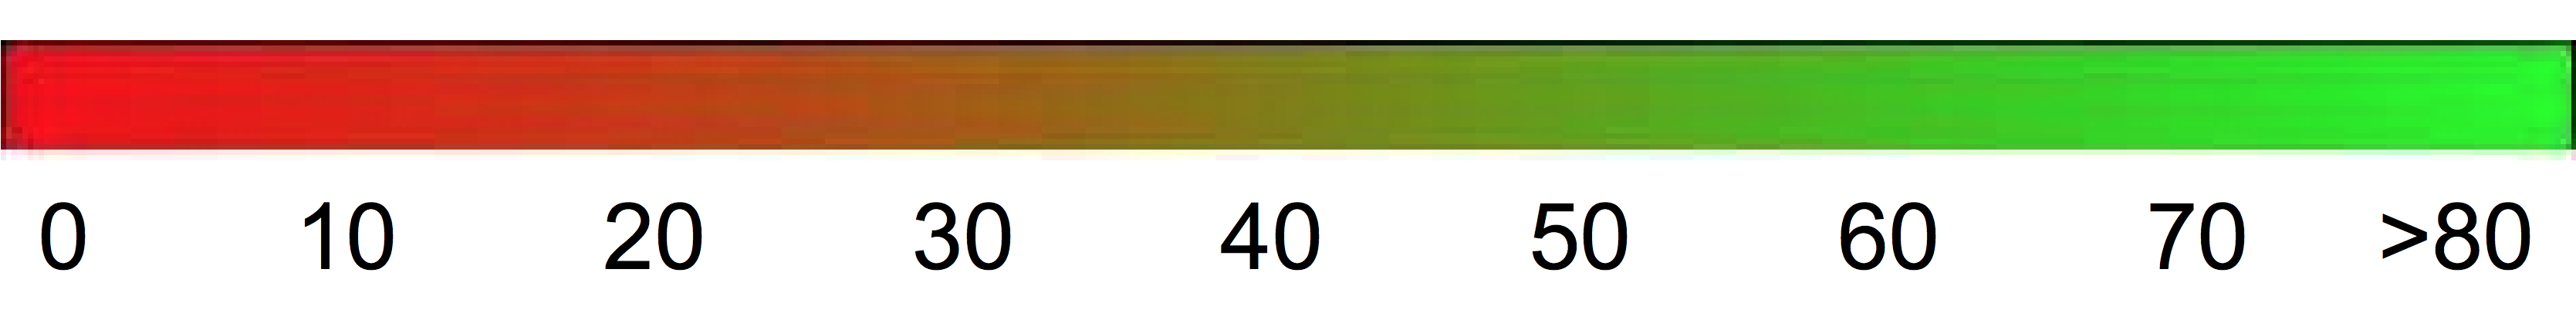
\includegraphics[width=\textwidth,keepaspectratio]{figures/bleu_score_range.png}
    \caption{Gradient for interpreting BLEU score \textcite{lavie2011evaluating}.}
    \label{fig:bleu}
\end{figure}
The method is based on n-gram matching, where n-grams in the reference translation are matched against n-grams in the translation. The matches are position-independent. The more matches, the higher the score.\\

\noindent For example, consider the following two translations:\\

\indent Candidate: \underline{on} \underline{the} \underline{mat} \underline{the} \underline{cat} sat.\\
\indent Reference: \underline{The} \underline{cat} is \underline{on} \underline{the} \underline{mat}.\\

\noindent The unigram precision \(\left(p_1\right) = 5/6\)\\

\noindent However, machine translations tend to generate an abundance of reasonable words, which could result in an inaccurately high precision. To combat this, \acrshort{bleu} uses something called modified precision\cite{papineni2002bleu}. The modification consists of clipping the occurrence of an n-gram to the maximum number the n-gram occurs in the reference. These clipped precision scores \(\left(p_n\right)\) are then calculated for n-grams up to length \(N\), normally 1-grams through 4-grams. They are then combined by computing the geometric average precision, as shown in \cref{eq:geometric-average-precision}. In addition, positive weights \(w_n\) are used, normally set to \(w_n = 1/N\).

\begin{equation}
    \label{eq:geometric-average-precision}
    \text{Geometric Average Precision $\left(N\right)$} = \exp \left( \sum_{n=1}^{N} w_n \log{p_n} \right)
\end{equation}

\noindent \acrshort{bleu} also introduces a brevity penalty for penalizing translations that are shorter than the reference:

\begin{equation}
    \label{eqn:brevity-penalty}
    \text{Brevity Penalty} = 
    \begin{cases}
        1 & \text{if } c > r\\
        e^{\left(1-r/c \right)} & \text{if } c \le r
    \end{cases}
\end{equation}

\noindent The final \acrshort{bleu} score is then computed as:

\begin{equation}
    \label{eqn:bleu}
    \textsc{Bleu} = \text{Brevity Penalty} \cdot \text{Geometric Average Precision Scores $\left(N\right)$}
\end{equation}

\subsection{String metric}
\label{sec:string-metric}

\subsubsection{Jaccard index}
\label{sec:jaccard-index}
The Jaccard index \cite{jaccard} is also known as the Jaccard similarity coefficient. It is a statistic used for gauging the similarity of sample sets. It is defined as the size of the intersection divided by the size of the union of the sets, as shown in \cref{eqn:jaccard}.

\begin{equation}
    \label{eqn:jaccard}
    J(A,B)=\frac{|A \cap B|}{|A \cup  B|}
\end{equation}

The Jaccard index ranges from 0 to 1. The higher the number, the more similar the two sets are.

The Jaccard index can for example be used as a measure of how similar two text strings are. For this, the strings are simply converted into sets of n-grams. The n-grams are then compared using the Jaccard index.

\section{Blockchain}
\label{sec:blockchain}
Blockchain technology was popularized by Satoshi Nakamoto in 2008 with his publication of the article "Bitcoin: A Peer-to-Peer Electronic Cash System". He introduced the formal idea of a peer-to-peer electronic cash system based on blockchain. This made it possible for users to conduct transactions without any need for a central authority. A blockchain is a growing list of records linked together with the help of a cryptographic hash. Each of these records is called a block. The blocks contain a cryptographic hash of the previous block, transactional data, and a timestamp. Since all blocks contain the hash of the previous block, they end up forming a chain. To tamper with a block in the chain, this also requires altering all subsequent blocks. Because of this, Blockchains are resistant to modification. The longer the chain, the more secure it is.

%Several other blockchains have evolved from Bitcoin. Ethereum is one of the more popular.

\section{Smart Contract}
\label{sec:smart-contract}
The term "\acrlong{sc}" was introduced with the Ethereum platform in 2014. A \acrfull{sc} is a program that is executed on a blockchain. This enables non-trusting parties to create an \textit{agreement}. \acrshortpl{sc} have enabled several interesting new concepts, such as \acrfull{nft} and entirely new business models. Ever since Ethereum's introduction of \acrshortpl{sc}, the platform has kept its position as one of the most popular \acrshort{sc} blockchain platforms. Ethereum is an open, decentralized platform that allows users to create, store, and transfer digital assets. Solidity is the primary programming language that is used to write these \acrshortpl{sc} for Ethereum. Solidity is compiled down to bytecode, which is then deployed and stored on the blockchain. Ethereum also introduces the concept of gas. Ethereum describes gas as follows: \textquote{It is the fuel that allows it to operate, in the same way that a car needs gasoline to run \cite{ethereum2021gas}}. The gas is used to pay for the cost of executing a \acrshort{sc}. This also protects against malicious actors spamming the network \cite{ethereum2021gas}. The gas is paid in Wei, which is the smallest denomination of Ether. Due to the immutable nature of blockchain technology, once a smart contract is deployed, it cannot be changed. This can have serious security implications, as vulnerable contracts can not be updated.

\subsection{Smart Contract Security Vulnerabilities}
\label{sec:smart-contract-vulnerabilities}
There are many vulnerabilities in \acrfullpl{sc} that can be exploited by malicious actors. Throughout the last years, an increase in the use of the Ethereum network has led to the development of \acrshortpl{sc} that are vulnerable to attacks. Due to the nature of blockchain technology, the attack surface of \acrshortpl{sc} is somewhat different from that of traditional computing systems. The Smart Contract Weakness Classification (SWC) Registry \footnote{\url{https://swcregistry.io}} collects information about various vulnerabilities. Following is a list of the most common vulnerabilities in \acrlongpl{sc}:

\subsubsection{Integer Overflow and Underflow}
When an arithmetic operation reaches the maximum or minimum size of a certain data type, an integer overflow or underflow occurs. For example, adding or multiplying two integers may result in a value that is unexpectedly small. Considering the opposite, subtracting from a small integer may result in an unexpectedly large positive value. For example, an 8-bit integer addition 255 + 2 might result in 1.

\subsubsection{Transaction-Ordering Dependence}
There is no guarantee on the execution order of transactions in blockchain systems. A miner can influence the outcome of a transaction due to its own reordering criteria. For example, a transaction that is dependent on another transaction to be executed first may not be executed. This can be exploited by malicious actors, and is called transaction-ordering dependence, or TOD.

\subsubsection{Broken Access Control}
Access Control issues are common in most computer systems, not just smart contracts. However, because of the monetary nature and transparency of \acrshortpl{sc}, properly enforcing access controls are essential. Broken access control can for example occur due to wrong visibility settings of functions. This gives attackers a relatively straightforward way to access contracts' private assets. However, the bypass methods are sometimes more subtle. For example, in Solidity, reckless use of \lstinline[language=Solidity]!delegatecall! in proxy libraries, or use of the deprecated \lstinline[language=Solidity]!tx.origin! might result in broken access control. \cref{lst:broken-access-control} shows a simple Solidity contract where anyone can trigger the contract's self-destruct, which makes the code vulnerable. Due to its severity, unprotected self-destructs are also recognized as a separate vulnerability, named unprotected suicide.

\begin{lstlisting}[
    caption={Access control vulnerable Solidity \acrlong{sc} code},
    label=lst:broken-access-control,
    language=Solidity]s
contract SimpleSuicide {
    function sudicideAnyone() {
        selfdestruct(msg.sender);
    }
}
\end{lstlisting}

\subsubsection{Timestamp Dependency}
If a \acrlong{sc} is dependent on the timestamp of a transaction, it is vulnerable to attack. A miner has full control over the execution environment for a \acrshort{sc}. If the \acrshort{sc} platform allows for \acrshortpl{sc} to use the time defined by the execution environment, this may result in a vulnerability. An example of vulnerable use is a timestamp used as part of the conditions to perform any critical operation (e.g., sending ether) or as the source of entropy to generate random numbers. Hence, a malicious miner could gain an advantage by choosing a suitable timestamp for a block he is mining. \cref{lst:timestamp-dependency} shows an example Solidity \acrshort{sc} that contains this vulnerability. Here, the timestamp (the \lstinline[language=Solidity]!now! keyword on line 10) is used as a source of entropy to generate a random number.

\begin{lstlisting}[
    caption={Timestamp Dependency vulnerable Solidity \acrlong{sc} code},
    label=lst:timestamp-dependency,
    language=Solidity]
contract Roulette {
    uint public prevBlockTime; // One bet per block
    constructor() external payable {} // Initially fund contract
    
    // Fallback function used to make a bet
    function () external payable {
        require(msg.value == 5 ether); // Require 5 ether to play
        require(now != prevBlockTime); // Only 1 transaction per block
        prevBlockTime = now;
        if(now % 15 == 0) { // winner
            msg.sender.transfer(this.balance);
        }
    }
}
\end{lstlisting}

\subsubsection{Reentrancy}
Reentrancy is a vulnerability that occurs when a \acrshort{sc} calls an external contract. Most blockchain platforms that implement \acrshortpl{sc} provide a way to make external contract calls. In Ethereum, an attacker may carefully construct a \acrshort{sc} at an external address that contains malicious code in its fallback function. Then, when a contract sends funds to the address, it will invoke the malicious code. Usually, the malicious code triggers a function in the vulnerable contract, performing operations not expected by the developer. The name "reentrancy" comes from the fact that the external malicious contract calls a function on the vulnerable contract and the code execution then "reenters" it. \cref{lst:reentrancy} shows a Solidity \acrshort{sc} function where a user can withdraw all the user's funds from a contract. If a malicious actor creates a contract that calls the withdrawal function several times before completing, the actor would successfully withdraw more funds than the current available balance. This vulnerability could easily be eliminated by moving the updating of the balance on line 4 to above the transferring of funds on line 3.

\begin{lstlisting}[
    caption={Reentrancy vulnerable Solidity \acrlong{sc} code},
    label=lst:reentrancy,
    language=Solidity]
function withdraw() external {
    uint256 amount = balances[msg.sender];
    require(msg.sender.call.value(amount)());
    balances[msg.sender] = 0;
}   
\end{lstlisting}



%\section{Vulnerability detection methods and tools}
%\label{sec:vulnerability-detection-methods-and-tools}
%\todo{Condence into one section, describing the different methods.. Add ontology based detection (for SolDetector)}

%Over the years, many tools have been developed for the purpose of detecting vulnerabilities. This includes symbolic execution, syntax analysis, abstract interpretation, data flow analysis, fuzzy testing, and machine learning. In the following sections, these methods are briefly explained.

%\subsection{Symbolic execution}
%\label{sec:symbolic-execution}
%Symbolic execution is a method for analyzing a computer program to determine what inputs cause each part of a program to execute. Symbolic execution requires the program to run. During the execution of the program, symbolic values are used instead of concrete values. The program execution arrives at expressions in terms of symbols for expressions and variables, as well as constraints expressed as symbols for each possible outcome of each conditional branch of the program. Finally, the possible inputs, expressed as symbols, that trigger a branch can be determined by solving the constraints.

%%\subsubsection{Syntax analysis}
%\label{sec:syntax-analysis}
%Syntax analysis is a technique for analyzing computer programs by analyzing the syntactical features of a computer program. This usually involves some kind of pattern matching where the source code is first parsed into a tree structure. This tree is then analyzed by looking for vulnerable patterns while traversing the tree.

%\subsubsection{Abstract interpretation}
%\label{sec:abstract-interpretation}
%Abstract interpretation is a method to analyze computer programs by soundly approximating the semantics of a computer program. This results in a superset of the concrete program semantics. Normally, this is then used to automatically extract information about the possible executions of computer programs.

%\subsubsection{Data flow analysis}
%\label{sec:data-flow-analysis}
%Data flow analysis is a method for analyzing computer programs by gathering information about the flow of data through the source code. This is done by collecting all the possible set of values calculated at different points through a computer program. This method is able to analyze large programs, compared to, for example, symbolic execution.

%\subsubsection{Fuzzy testing}
%\label{sec:fuzzy-testing}
%Fuzzing is an automated testing technique for analyzing computer programs. The technique involves supplying invalid, unexpected, or random data inputs to a program in order to uncover bugs. The program is then monitored during execution for unexpected behavior such as crashes, errors, or failing built-in code assertions.
